% Generated by analyze_t2.js - paste before \end{document}
\subsection{T2 -- Offered load and saturation}
Executed on 2026-10-20 (17:05--17:47 CEST) with the benchmark harness acting as an
open-loop load generator (fixed inter-arrival times, 32 client connections per identity; requests are
released on schedule without waiting for previous responses). Offered rates 10, 20, 40, 80, 160, 320, 640, 1280\,TPS; for each
rate 3 repetitions of 15\,s warm-up, 30\,s measurement window and up to
30\,s drain. Only requests \emph{submitted} in the measurement window are counted; throughput and
goodput are averages over the window. The state-changing workload is \texttt{RegisterProduction} (independent keys,
includes the \texttt{userauth} authorization call, no prepared assets required); the read-only workload is
\texttt{VerifyByUID} on 50 prepared bound UIDs. A workload sweep stops after two consecutive
non-sustainable rates. \texttt{BatchTimeout} = 2\,s, \texttt{MaxMessageCount} = 10. Intermediate rates were added in a second session on 2026-10-21 (write: 160, 200, 240, 280, 320\,TPS, 08:23--08:31 CEST; read: 320, 360, 400, 480\,TPS, 08:43--08:50 CEST) on a freshly re-created network with the same configuration, using the P95 reference of the first session (write 946.3\,ms, read 18.4\,ms) for the saturation criterion. One rate per workload was repeated in both sessions as an anchor: state-changing 160\,TPS, goodput 160.0 vs 160.0\,TPS, P95 110.7 vs 352.7\,ms; read-only 320\,TPS, goodput 320.0 vs 320.0\,TPS, P95 16.9 vs 14.7\,ms (first vs second session).

\begin{table}[H]
\centering\small
\caption{T2: offered load sweep (mean over 3 repetitions; goodput $\pm$ 95\% CI). $\lambda$: measured
submission rate; goodput: valid transactions per second; latency percentiles of valid requests; CPU: mean of the two
peers and of the orderer in \% of one core during the measurement window; sustainable: saturation criterion of
Section~2.5 satisfied in every repetition.}
\label{tab:t2}
\setlength{\tabcolsep}{3.5pt}
\begin{tabular}{rrrrrrrrrc}
\toprule
Offered & $\lambda$ & Goodput & P50 & P95 & P99 & Fail & CPU peer & CPU ord. & Sust. \\
(TPS) & (TPS) & (TPS) & (ms) & (ms) & (ms) & (\%) & (\%) & (\%) & \\
\midrule
\multicolumn{10}{l}{\emph{State-changing (\texttt{RegisterProduction})}} \\
10 & 10.0 & 10.0 $\pm$ 0.0 & 497.4 & 946.3 & 950.2 & 0.00 & 9.3 & 2.0 & yes \\
20 & 20.0 & 20.0 $\pm$ 0.0 & 258.5 & 479.9 & 487.1 & 0.00 & 11.6 & 2.3 & yes \\
40 & 40.0 & 40.0 $\pm$ 0.0 & 147.3 & 255.5 & 260.0 & 0.00 & 20.8 & 5.0 & yes \\
80 & 80.0 & 80.0 $\pm$ 0.0 & 89.0 & 143.9 & 147.3 & 0.00 & 44.0 & 10.6 & yes \\
160 & 160.0 & 160.0 $\pm$ 0.0 & 78.7 & 110.7 & 120.7 & 0.00 & 129.1 & 34.6 & yes \\
200 & 200.3 & 200.3 $\pm$ 1.4 & 4584.3 & 5832.4 & 5965.9 & 0.00 & 153.7 & 46.3 & no \\
240 & 240.0 & 240.0 $\pm$ 8.9 & 22896.6 & 31719.3 & 32664.3 & 0.00 & 141.9 & 39.2 & no \\
320 & 318.1 & 318.1 $\pm$ 12.5 & 32410.6 & 39914.7 & 40969.1 & 0.00 & 136.8 & 34.7 & no \\
640 & 651.3 & 0.5 $\pm$ 2.1 & 49502.2 & 56722.1 & 56886.1 & 99.93 & 170.2 & 13.2 & no \\
\multicolumn{10}{l}{\emph{Read-only (\texttt{VerifyByUID})}} \\
10 & 10.0 & 10.0 $\pm$ 0.0 & 14.2 & 18.4 & 21.3 & 0.00 & 4.8 & 0.1 & yes \\
20 & 20.0 & 20.0 $\pm$ 0.0 & 15.7 & 19.0 & 22.1 & 0.00 & 9.2 & 0.1 & yes \\
40 & 40.0 & 40.0 $\pm$ 0.0 & 11.6 & 15.2 & 16.9 & 0.00 & 14.5 & 0.1 & yes \\
80 & 80.0 & 80.0 $\pm$ 0.0 & 6.6 & 9.0 & 11.1 & 0.00 & 16.3 & 0.0 & yes \\
160 & 160.0 & 160.0 $\pm$ 0.0 & 7.2 & 9.1 & 11.0 & 0.00 & 31.7 & 0.1 & yes \\
320 & 320.0 & 320.0 $\pm$ 0.0 & 10.9 & 16.9 & 24.0 & 0.00 & 64.6 & 0.1 & yes \\
360 & 360.0 & 360.0 $\pm$ 0.0 & 13.4 & 71.0 & 131.2 & 0.00 & 69.2 & 0.1 & no \\
400 & 400.0 & 400.0 $\pm$ 0.0 & 2185.7 & 4269.4 & 4382.8 & 0.00 & 82.3 & 0.1 & no \\
640 & 640.0 & 0.0 $\pm$ 0.0 & -- & -- & -- & 100.00 & 111.5 & 0.1 & no \\
1280 & 1149.0 & 0.0 $\pm$ 0.0 & -- & -- & -- & 100.00 & 88.6 & 0.1 & no \\
\bottomrule
\end{tabular}
\end{table}

\begin{figure}[H]
\centering
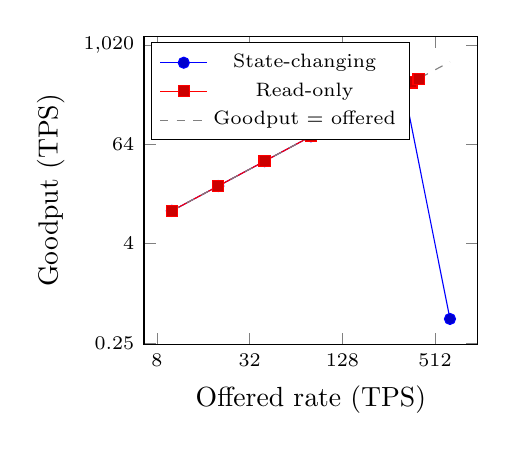
\begin{tikzpicture}
\begin{axis}[width=0.48\linewidth, height=5.5cm, xmode=log, log basis x=2, ymode=log, log basis y=2,
  xlabel={Offered rate (TPS)}, ylabel={Goodput (TPS)}, log ticks with fixed point, tick label style={font=\scriptsize},
  legend style={font=\scriptsize, at={(0.02,0.98)}, anchor=north west}]
\addplot+[mark=*] coordinates {(10,10.00) (20,20.00) (40,40.00) (80,80.00) (160,160.00) (200,200.26) (240,239.98) (320,318.07) (640,0.49)};
\addlegendentry{State-changing}
\addplot+[mark=square*] coordinates {(10,10.00) (20,20.00) (40,40.00) (80,80.00) (160,160.00) (320,320.00) (360,360.00) (400,400.00)};
\addlegendentry{Read-only}
\addplot[dashed, gray] coordinates {(10,10) (20,20) (40,40) (80,80) (160,160) (200,200) (240,240) (320,320) (640,640)};
\addlegendentry{Goodput = offered}
\end{axis}
\end{tikzpicture}\hfill
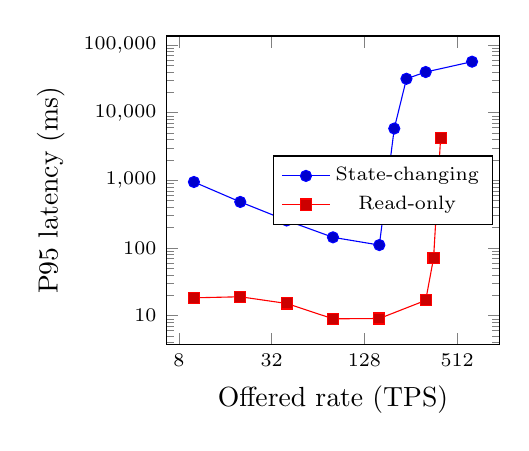
\begin{tikzpicture}
\begin{axis}[width=0.48\linewidth, height=5.5cm, xmode=log, log basis x=2, ymode=log,
  xlabel={Offered rate (TPS)}, ylabel={P95 latency (ms)}, log ticks with fixed point, tick label style={font=\scriptsize},
  legend style={font=\scriptsize, at={(0.98,0.5)}, anchor=east}]
\addplot+[mark=*] coordinates {(10,946.25) (20,479.91) (40,255.52) (80,143.93) (160,110.68) (200,5832.42) (240,31719.31) (320,39914.69) (640,56722.13)};
\addlegendentry{State-changing}
\addplot+[mark=square*] coordinates {(10,18.38) (20,19.05) (40,15.16) (80,9.00) (160,9.09) (320,16.86) (360,71.04) (400,4269.40)};
\addlegendentry{Read-only}
\end{axis}
\end{tikzpicture}
\caption{T2: goodput (left) and P95 latency (right) as a function of the offered rate (logarithmic axes).}
\label{fig:t2}
\end{figure}

\paragraph{Observations.}
\begin{itemize}
  \item \textbf{State-changing workload:} the highest sustainable offered rate was 160\,TPS (goodput 160.0\,TPS, P95 110.7\,ms); the criterion was first violated at 200\,TPS (P95>2*base, backlog growing), where the goodput reached 200.3\,TPS.
  \item \textbf{Read-only workload:} the highest sustainable offered rate was 320\,TPS (goodput 320.0\,TPS, P95 16.9\,ms); the criterion was first violated at 360\,TPS (P95>2*base), where the goodput reached 360.0\,TPS.
  \item \textbf{Latency under load.} For state-changing transactions the latency first \emph{decreases} with the offered
        rate, because blocks reach \texttt{MaxMessageCount} = 10 before the 2\,s \texttt{BatchTimeout} expires (T1-b), and
        increases again only when the system approaches saturation.
  \item \textbf{Storage under load.} The 93983 valid \texttt{RegisterProduction} transactions of the sweep
        added 548.0\,MB of block files, 27.7\,MB of world state and
        6.1\,MB of history database per peer, i.e.\ 6.34\,KB per transaction
        (5.97\,KB of block files) with batched blocks.
  \item \textbf{Scope.} The load generator runs on the same host as the network; the reported capacity is therefore a
        lower bound for the tested single-host configuration and not a property of Fabric or of Enhanced SPECTRA in
        general.
\end{itemize}
